\documentclass{standalone}
\usepackage{ tikz }
\usepackage{ xparse }
\input{macros/all}

\begin{document}
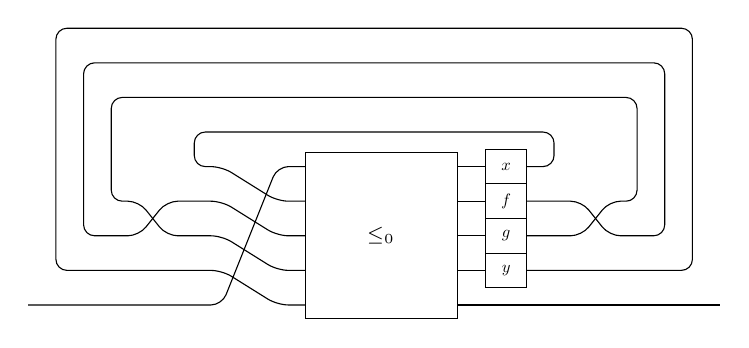
\begin{tikzpicture}[yscale=-1,x=1em,y=1.25em]

    \draw[rounded corners] (16, 9) -- (22, 9) -- (22, 2) -- (-1, 2) -- (-1, 9) -- (5, 9) -- (7, 10) -- (8, 10);
    \draw[rounded corners] (16, 8) -- (18, 8) -- (19, 7) -- (20, 7) -- (20, 4) -- (1, 4) -- (1, 7) -- (2, 7) -- (3, 8) -- (5, 8) -- (7, 9) -- (8, 9);
    \draw[rounded corners] (16, 7) -- (18, 7) -- (19, 8) -- (21, 8) -- (21, 3) -- (0, 3) -- (0, 8) -- (2, 8) -- (3, 7) -- (5, 7) -- (7, 8) -- (8, 8);
    \draw[rounded corners] (16, 6) -- (17, 6) -- (17, 5) -- (4, 5) -- (4, 6) -- (5, 6) -- (7, 7) -- (8, 7);

    \draw[rounded corners] (-2, 10) -- (5, 10) -- (7,6) -- (8,6);

    \node[draw, minimum height = 6em, minimum width = 5.5em, anchor = west] at (8, 8){$\shuffle_{\leq_0}$};

    \draw[rounded corners] (13.5, 6) -- (14.5, 6);
    \draw[rounded corners] (13.5, 7) -- (14.5, 7);
    \draw[rounded corners] (13.5, 8) -- (14.5, 8);
    \draw[rounded corners] (13.5, 9) -- (14.5, 9);
    \draw[rounded corners] (13.5, 10) -- (23, 10);

    \node[draw, minimum height = 1.25em, minimum width = 1.5em, anchor = west] at (14.5,6){\scalebox{0.6}{$x$}};
    \node[draw, minimum height = 1.25em, minimum width = 1.5em, anchor = west] at (14.5,7){\scalebox{0.6}{$f$}};
    \node[draw, minimum height = 1.25em, minimum width = 1.5em, anchor = west] at (14.5,8){\scalebox{0.6}{$g$}};
    \node[draw, minimum height = 1.25em, minimum width = 1.5em, anchor = west] at (14.5,9){\scalebox{0.6}{$y$}};

\end{tikzpicture}
\end{document}